\let\negmedspace\undefined
\let\negthickspace\undefined
\documentclass[journal]{IEEEtran}
\usepackage[a5paper, margin=10mm, onecolumn]{geometry}
\usepackage{lmodern} % Ensure lmodern is loaded for pdflatex
\usepackage{tfrupee} % Include tfrupee package

\setlength{\headheight}{1cm} % Set the height of the header box
\setlength{\headsep}{0mm}     % Set the distance between the header box and the top of the text

\usepackage{gvv-book}
\usepackage{gvv}
\usepackage{cite}
\usepackage{amsmath,amssymb,amsfonts,amsthm}
\usepackage{algorithmic}
\usepackage{graphicx}
\graphicspath{{./figs/}}
\usepackage{textcomp}
\usepackage{xcolor}
\usepackage{txfonts}
\usepackage{listings}
\usepackage{enumitem}
\usepackage{mathtools}
\usepackage{gensymb}
\usepackage{comment}
\usepackage{float}
\usepackage[breaklinks=true]{hyperref}
\usepackage{tkz-euclide} 
\def\inputGnumericTable{}                                 
\usepackage[latin1]{inputenc}                                
\usepackage{color}                                            
\usepackage{array}                                            
\usepackage{longtable}                                       
\usepackage{calc}                                             
\usepackage{multirow}                                         
\usepackage{hhline}                                           
\usepackage{ifthen}                                           
\usepackage{lscape}
\usepackage{circuitikz}
\tikzstyle{block} = [rectangle, draw, fill=blue!20, 
text width=4em, text centered, rounded corners, minimum height=3em]
\tikzstyle{sum} = [draw, fill=blue!10, circle, minimum size=1cm, node distance=1.5cm]
\tikzstyle{input} = [coordinate]
\tikzstyle{output} = [coordinate]


\begin{document}
	
	\bibliographystyle{IEEEtran}
	\vspace{3cm}
	
	\title{1.5.4}
	\author{EE25BTECH11016 - Taraka Abhinav}
	\maketitle
	{\let\newpage\relax\maketitle}
	
	\setlength{\intextsep}{10pt} % Space between text and floats

\textbf{Question:}\\
A circle has its center at $(4,4)$. If one end of a diameter is $(4,0)$, then find the coordinates of the other end.\\
\solution\\
Let the position vectors for the center, the known end, and the unknown end of the diameter be $\vec{C}$, $\vec{B}$, and $\vec{A}$ respectively. Let the coordinates of the unknown end $\vec{A}$ be $(a,b)$.

The given vectors are:
\begin{align}
\vec{A} = \myvec{a\\b}, \quad \vec{B} = \myvec{4\\0}, \quad \vec{C} = \myvec{4\\4}
\end{align}

The center of the circle is the midpoint of the diameter. Therefore, the center vector is the average of the endpoint vectors.
\begin{align}
\vec{C} = \frac{\vec{A}+\vec{B}}{2}
\end{align}

To find the unknown vector $\vec{A}$, we rearrange the equation:
\begin{align}
2\vec{C} &= \vec{A} + \vec{B} \\
\vec{A} &= 2\vec{C} - \vec{B}
\end{align}

Substituting the given vector values:
\begin{align}
\myvec{a\\b} &= 2\myvec{4\\4} - \myvec{4\\0} \nonumber \\
&= \myvec{8\\8} - \myvec{4\\0} \\
&= \myvec{4\\8}
\end{align}

\[ \therefore \text{The other end of the diameter is }(4,8). \]

\begin{figure}[H]
    \centering
    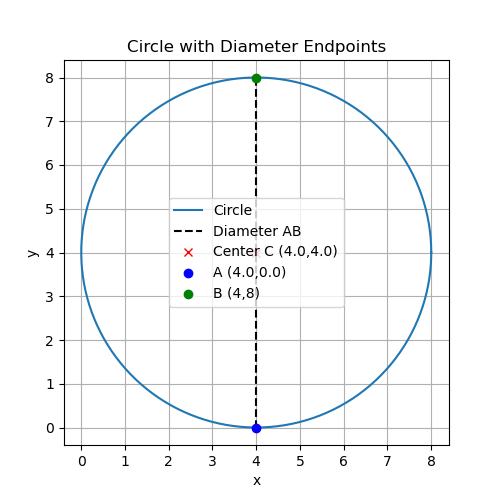
\includegraphics[width=0.5\linewidth]{figs/Figure_1.png}
    \label{fig:circle}
\end{figure}

\end{document}